\newpage
\section{Homoskedasticity and Heteroskedasticity}

In this section we wish to introduce \homo and \hetero. The section is based on \cite{Wooldridge2012}. First we define what \homo and \hetero is. 

\begin{definition}[Homoskedasticity and heteroskedasticity]
When the variance of the error term does not depend on the explanatory variables $\mathbf{X}$ and is constant, the errors is said to be homoscedastic, thus the errors should satisfy
\begin{align*}
    \var(\varepsilon | \mathbf{X}) = \var(\varepsilon) = \sigma^2
\end{align*}
If this is not satisfied the error is said to be heteroskedastic. 

\end{definition}

The intuition behind \homo is that the variance of the error does not depend on the explanatory variables $\mathbf{X}$, hence it does not change for any value given to the explanatory variables. Conversely if the variance of the error term changes with any of the explanatory variables the error term is heteroskedastic. 

Homoskedasticity and \hetero can be illustrated as in figure \ref{fig:homo_with_dependent_up_axis} and \ref{fig:hetero_with_dependent_up_axis}. 
\begin{figure}[h]
\centering
\begin{subfigure}[b]{0.5\textwidth}
    \centering
    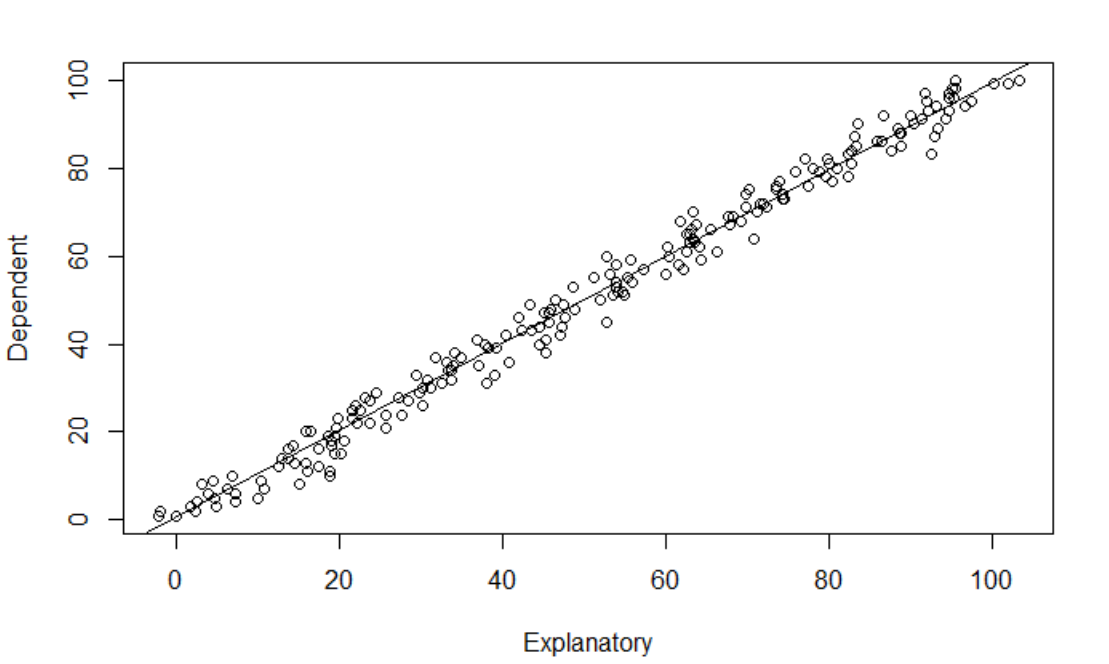
\includegraphics[width = \textwidth]{figures/Thea/homoplot.png}
    \caption{\homo}
    \label{fig:homo_with_dependent_up_axis}
\end{subfigure}%
\begin{subfigure}[b]{0.5\textwidth}
\centering
    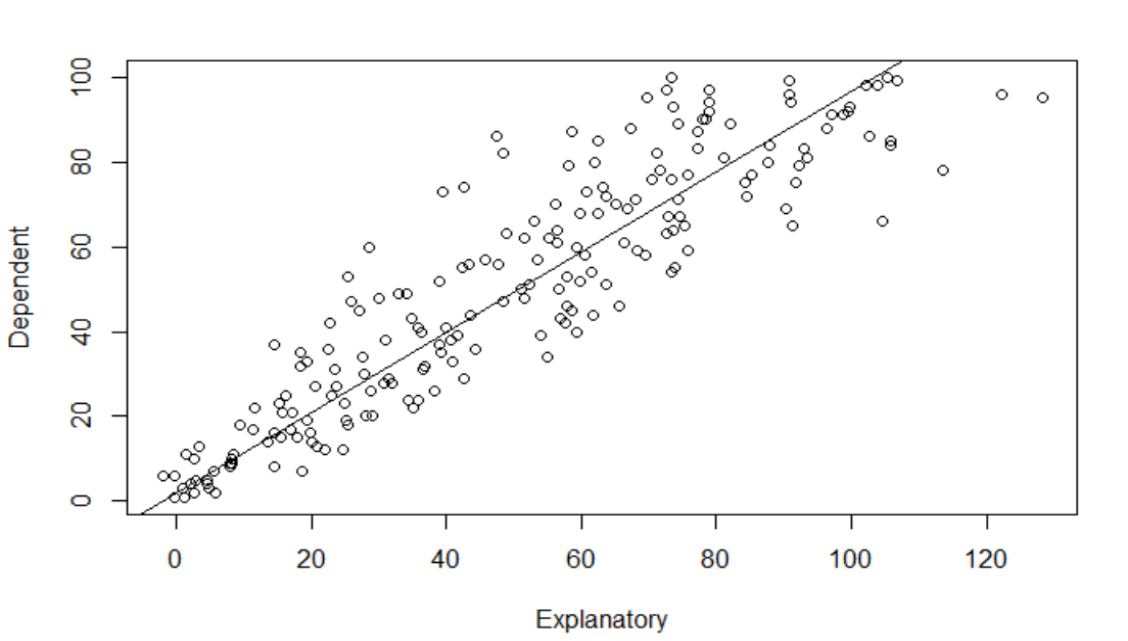
\includegraphics[width = \textwidth]{figures/Thea/Heteroplot.png}
    \caption{\hetero}
    \label{fig:hetero_with_dependent_up_axis}
\end{subfigure}
\end{figure}
In the case of \homo the variance is consistent for all values of $\mathbf{X}$, to which the standard errors do not depend on the explanatory variables.
In the case of \hetero the variance changes as $\mathbf{X}$ changes. Typically the variance becomes greater as $\mathbf{X}$ becomes greater.

For an example you can consider a households income and its spending on luxury items. If the income is low most will be spend on necessity items such as food. If the income is high there is the possibility but not the guarantee of spending more on luxury items, thus there will be a greater variance in the consumption of luxury goods in the segment with higher household income. Heteroskedasticity can arise when variances of unobserved factors changes over different segments in the sample space. 

It is desired to have \homo rather than \hetero because \hetero will cause problems in statistical tests and linear regression, which will be investigated further in the next section. 

\subsection{Consequences of \hetero}
In this sections we wish to determine how \hetero will affect both OLS, \textit{t-statistics}, \textit{F-statistics} and \textit{confidence intervals}. 

First we wish to determine if the estimator $\betahat$ is unbiased or biased in the presence of heteroskedasticity.  

Remember assumption \ref{as:linear_in_the_parameters}, \ref{as:no_perfect_collinearity} and \ref{as:zero_conditional_mean}. If these hold theorem \ref{th:unbiasedness_of_ols} proved that the OLS estimator $\betahat$ is unbiased for $\boldsymbol{\beta}$, which is the same as $E[\hat{\beta}_j] = \beta_j
$ for $j = 1,2, \ldots, k$. 

Because the error terms in $\var(\boldsymbol{\varepsilon} | \mathbf{X})$ did no determine whether the OLS was biased or unbiased in the theorem and its proof, the presence of \hetero will not cause $\betahat$ to be biased. 

Next we wish to determine how our measure-of-fit test $\mathcal{R}^2$ is influenced by \hetero. 

$\mathcal{R}^2$ measures how much of the variance in the dependent variable is explained by the independent variables. In our model it determines how much of the variance in $y$ is explained in the variables $\mathbf{X}$. 
Low values of $\mathcal{R}^2$ makes predictions difficult because most of the variance in $y$ is caused by unobserved factors in $\varepsilon$, so the OLS predictions will be hard to calculate given a set of explanatory variables.
Consider the expression for $\mathcal{R}^2$
\begin{align*}
    \mathcal{R}^2 = 1 - \dfrac{SSR}{SST}
\end{align*}
Where \textbf{SSR} is the \textbf{sum of squared residuals} given as
\begin{align*}
    SSR \equiv \nsum \hat{\varepsilon}_i^2
\end{align*}
and \textbf{SST} is the \textbf{total sum of squares} given as
\begin{align*}
    SST \equiv \nsum (y_i - \overline{y})^2. 
\end{align*}
The $\mathcal{R}^2$ value is between $0$ and $1$. The closer the value is to one $1$ the more of the variance is accounted for in the explanatory variables, thus it is desireable to have an $\mathcal{R}^2$ value close to $1$.
This coefficient of determination can be changed to the adjusted $\mathcal{R}^2$ as
\begin{align*}
    \mathcal{R}^2_{Adj} = 1 - \dfrac{SSR/(n - k - 1)}{SST/(n - 1)}
\end{align*}
This rewriting of the model adjusts for the number of predictors in the model. This $\mathcal{R}^2$ in- and decreases if a predictor improves more or less than expected, respectively. 

Both SSR and SST are unconditional variances in $\mathcal{R}^2$, thus they are not influenced by the presence of \hetero.  

This means that \hetero does not cause the OLS estimators to be biased or inconsistent and nor does it affect the $\mathcal{R}^2$ test, however it will cause the variance of the OLS estimators, i.e. $\var(\betahat)$, to be biased, which will be explained next.  

The \homo assumption is $\var(\boldsymbol{\varepsilon} | \mathbf{X}) = \sigma^2$. If assumption \ref{as:linear_in_the_parameters}, \ref{as:no_perfect_collinearity}, \ref{as:zero_conditional_mean} and \ref{as:homoskedasticity_and_no_serial_correlation} hold the variance of the OLS estimator can be expressed as in theorem \ref{th:variance-covariance_of_the_ols_estimator}, which implies that variance of $\betahat$ given the explanatory variables has an explicit form given as
\begin{align*}
    \var(\betahat | \mathbf{X}) = \sigma^2(\mathbf{X}^\top\mathbf{X})^{-1}.
\end{align*}
The slope coefficients can be defined as 
\begin{align}\label{eq:slope_variance_OLS_estimator}
    \var(\hat{\beta}_j|\mathbf{X}) = \dfrac{\sigma^2}{SST_j(1- \mathcal{R}_j^2)}
\end{align}
Where $j = 1, \ldots, k$ and $SST_j = \nsum (x_{ij} - \overline{x}_j)^2$ is the total sample variation in $x_j$ and $\mathcal{R}^2_j$ is found from a regression on $x_j$ with all other independent variables. 

Equation \eqref{eq:slope_variance_OLS_estimator} depends on $\sigma^2$, $SST_j$ and $\mathcal{R}^2_j$.
Here $\sigma^2$ is an unknown variable, the larger $\sigma^2$ the larger are the variances for the OLS estimators. $SST_j$ is the total sample variation in $x_j$, the larger it is the smaller will the variance of the OLS estimators be so it is preferred to have as much sample variation as possible which can be obtained by increasing sample size. 
Notice that $\mathcal{R}^2_j$ is found with a regression involving only the independent variables in the original model, where $x_j$ is the dependent variable. This differs from the $\mathcal{R}^2$ found by regression on $y$ with $x_1, \ldots, x_k$ as the independent variables. 
Consider the example $y = \betahat_0 + \betahat_1 x_1 + \betahat_2 x_2 + \varepsilon$, here $\mathcal{R}^2_1$ is found by making a regression of $x_1$ on $x_2$. 
As always an $\mathcal{R}^2_1$ value close to one means that $x_2$ explains much of the variation in $x_1$, so a value close to $1$ means that $x_1$ and $x_2$ are highly correlated.
$\mathcal{R}^2_j$ tests how much of the variation in one of the independent variables is explained from the remaining independent variables.
The best estimator for $\betahat_j$ is found with a low value of $\mathcal{R}^2_j$, thus a smaller relationship between the explanatory variables is desired when retrieving $\var(\betahat_j)$. Note $\mathcal{R}^2$ cannot equal $0$ due to assumption \ref{as:no_perfect_collinearity}. 

From \eqref{eq:slope_variance_OLS_estimator} it is possible to find the standard deviation of $\betahat_j$, which is the squre root of \ref{eq:slope_variance_OLS_estimator}, which is
\begin{align}\label{eq:standard_deviation}
    sd(\betahat_j) = \dfrac{\sigma}{SST_j(\big(1- \mathcal{R}_j^2)\big)^{1/2}}
\end{align}
The standard deviation, $\sigma$, is replaced by its estimate to obtain the standard error
\begin{align}\label{eq:standad_error}
    se(\betahat_j) = \dfrac{\hat{\sigma}}{SST_j(\big(1- \mathcal{R}_j^2)\big)^{1/2}}
\end{align}
Note that the standard deviation measures the dispersion a data set has from the mean, whereas the standard errors measures how far the sample mean of the data is likely to be from the true sample space mean. 

Since \eqref{eq:standad_error} is obtained from \eqref{eq:slope_variance_OLS_estimator}, which relies on \homo the standard error will not be a valid estimator of the standard deviation in \eqref{eq:standard_deviation} in the presence of \hetero. This means that \hetero will cause bias in the $\var(\betahat_j)$ which invalidates the standard errors, $\varepsilon$. 

Furthermore \textit{confidence intervals}, \textit{t-statistics} and \textit{F-statistics} will no longer follow a normal distribution and thus their results will be invalid when \hetero is present. 


The OLS is the \textbf{best linear unbiased estimator (BLUE)}, if assumption  \ref{as:linear_in_the_parameters}, \ref{as:no_perfect_collinearity}, \ref{as:zero_conditional_mean} and \ref{as:homoskedasticity_and_no_serial_correlation} holds. In the Gauss-Markov theorem \ref{th:gauss_markoc_theorem}, it is seen that in order for the OLS to be the BLUE it is a necessary for the \homo assumption to hold true, otherwise it would not have the smallest variance of the estimators causing it to not be the best estimator.





\subsection{Correct for \hetero}
If we sum up \hetero will in general cause OLS standard errors to be faulty as well as the related statistical tests. In this section we wish to correct for these mistakes, so they are correct when \hetero is present. 


First it is needed to estimate the estimators of variance, $\var(\betahat)$, when \hetero is present. 


\subsection{test for \hetero}





% \newpage
% \section{Homoskedasticity and Heteroskedasticity}

% In this section we wish to introduce \homo and \hetero. The section is based on \cite{Wooldridge2012}. First we define what \homo and \hetero is. 

% \begin{definition}[Homoskedasticity and heteroskedasticity]
% When the variance of the error term does not depend on the explanatory variables $\mathbf{X}$ the errors is said to be homoskedastic, thus the errors should obey
% \begin{align*}
%     \var(\varepsilon | \mathbf{X}) = \var(\varepsilon) = \sigma^2
% \end{align*}
% If this is not satisfied the error is said to be heteroskedastic. 

% \end{definition}

% The intuition behind \homo is that the variance of the error does not depend on the explanatory variables $\mathbf{X}$, hence it does not change for any value given to the explanatory variables. Conversely if the variance of the error term changes with any of the explanatory variables the error term is \hetero. 

% Homoskedasticity and \hetero can be illustrated as in figure \ref{fig:homo_with_dependent_up_axis} and \ref{fig:hetero_with_dependent_up_axis}. 


% \begin{figure}[h]
% \centering
% \begin{subfigure}[b]{0.5\textwidth}
%     \centering
%     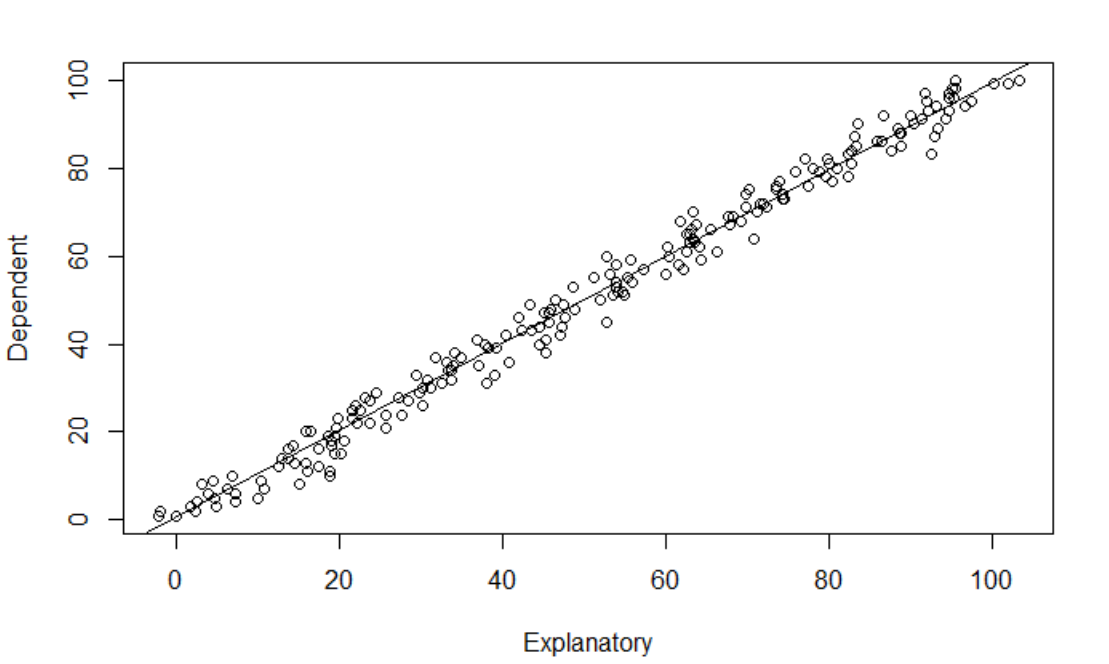
\includegraphics[width = \textwidth]{figures/Thea/homoplot.png}
%     \caption{\homo}
%     \label{fig:homo_with_dependent_up_axis}
% \end{subfigure}%
% \begin{subfigure}[b]{0.5\textwidth}
% \centering
%     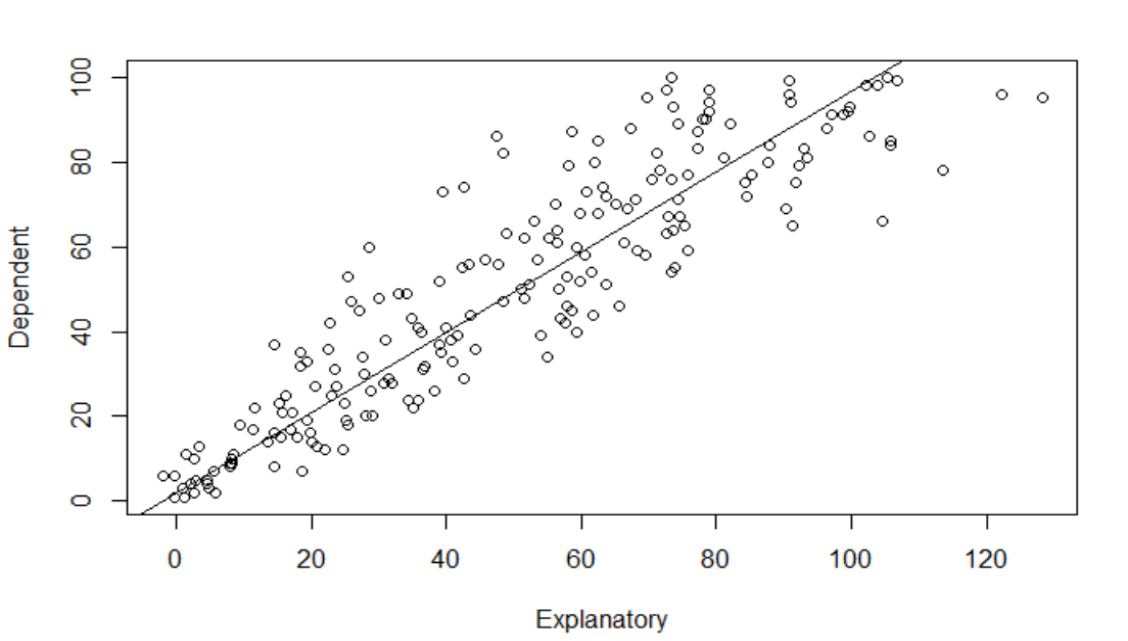
\includegraphics[width = \textwidth]{figures/Thea/Heteroplot.png}
%     \caption{\hetero}
%     \label{fig:hetero_with_dependent_up_axis}
% \end{subfigure}
% \end{figure}


% In the case of \homo the variance is consistent for all values of $\mathbf{X}$, to which the standard errors do not depend on the explanatory variables. In the case of \hetero the variance changes as $\mathbf{X}$ changes. Typically the variance becomes greater as $\mathbf{X}$ becomes greater.

% For an example you can consider a households income and its spending on luxury items. If the income is low most will be spend on necessity items such as food, if the income increases there is the possibility but not the necessity of spending more on luxury items, thus there will be a greater variance in the consumption of luxury goods the higher the household income is. In short \hetero  can arise when variances of unobserved factors changes over different segments in the sample space. 

% It is desired to have \homo rather than \hetero because \hetero will cause problems in statistical analysis, which will be explained in the next section. 






% \subsection{Consequences of \hetero}

% In this sections we wish to determine how \hetero will affect our statistical test related to the model.  

% First we wish to determine if $\betahat$ is unbiased or biased in general and in the presence of heteroskedasticity.  

% Remember assumption \ref{as:linear_in_the_parameters}, \ref{as:no_perfect_collinearity} and \ref{as:zero_conditional_mean}. If these hold theorem \ref{th:unbiasedness_of_ols} showed that the OLS estimator $\betahat$ is unbiased for $\boldsymbol{\beta}$, which is the same as $E[\betahat_j] = \beta_j$ for $j = 1,2, \ldots, k$. 












% % If the above mentioned assumptions holds true the OLS estimator $\betahat$ is  unbiased for $\beta$. This is the same as 

% % \begin{align*}
% %     E[\betahat_j] = \beta_j, \quad j = 1,2, \ldots, k
% % \end{align*}

% % where $\betahat_j$ is the parameter. 

% This can be proven, by first considering the expression for $\betahat$ which is given in \eqref{eq:equation_to} and rewriting as follows

% \begin{align*}
%     \betahat &= \left(\mathbf{X}^\top\mathbf{X}\right)^{-1}\mathbf{X}^\top\mathbf{y}\\
%     &= \left( \mathbf{X}^T\mathbf{X}\right)^{-1}\mathbf{X}^T\left( \mathbf{X}\mathbf{\beta} + \mathbf{\varepsilon}\right)\\
%     &= \left( \mathbf{X}^T\mathbf{X}\right)^{-1} \left( \mathbf{X}^T\mathbf{X}\right) \mathbf{\beta} + \left( \mathbf{X}^T\mathbf{X}\right)^{-1}\mathbf{X}^T\mathbf{\varepsilon}\\
%     &= \mathbf{\beta} + \left( \mathbf{X}^T\mathbf{X}\right)^{-1}\mathbf{X}^T\varepsilon
% \end{align*}

% If we then take the conditional expectation it gives

% \begin{align*}
%     E[\betahat | \mathbf{X}] &= \betahat + \left( \mathbf{X}^T \mathbf{X}\right)^{-1}\mathbf{X}^T E[\varepsilon | \mathbf{X}]\\
%     &= \betahat + \left( \mathbf{X}^T\mathbf{X}\right)^{-1}\mathbf{X}^T\mathbf{0}\\
%     &= \mathbf{\beta}
% \end{align*}

% Thus it is shown that $\betahat$ is unbiased. Because the error terms in $\varvarepsilon | \mathbf{X})$ did no determine whether the OLS was biased or unbiased the presence of \hetero will not cause $\betahat$ to be biased. 

% Next we wish to determine how our measure of fit test $\mathcal{R}^2$ is influenced by \hetero. 
% $\mathcal{R}^2$ measures how much of the variance in $y$ is explained in $\mathbf{X}$. Low values of $\mathcal{R}^2$ makes predictions difficult because most of the variance in $y$ is caused by unobserved factors, so the OLS predictions will be hard to calculate given a set of explanatory variables.
% Consider the expression for $\mathcal{R}^2$

% \begin{align*}
%     \mathcal{R}^2 = 1 - \dfrac{SSR}{SST}
% \end{align*}

% Where \textbf{SSR} is the \textbf{sum of squared residuals} given as

% \begin{align*}
%     SSR \equiv \nsum \hat{\varepsilon}_i^2
% \end{align*}


% and \textbf{SST} is the \textbf{total sum of squares} given as

% \begin{align*}
%     SST \equiv \nsum (y_i - \overline{y})^2. 
% \end{align*}

% The $\mathcal{R}^2$ value is between $0$ and $1$. The closer the value is to one $1$ the more of the variance is accounted for, thus it is beneficial to have an $\mathcal{R}^2$ value close to $1$. 

% If we define $\sigma^2_y$ as the variance of $y$ and define $\sigma^2_{\varvarepsilon}$ as the variance of the error term $\varvarepsilon$, the expression for the $\mathcal{R}^2$ test for our model becomes

% \begin{align*}
%     \mathcal{R}^2_{Model} = 1 - \dfrac{\sigma^2_{\varvarepsilon}}{\sigma^2_y}
% \end{align*}

% Which measures the how much of the variance in $y$ is explained by the explanatory variables $\mathbf{X}$. This model can be changed to the adjusted $\mathcal{R}^2$ as

% \begin{align*}
%     \mathcal{R}^2_{Model} = 1 - \dfrac{\sigma^2_{\varvarepsilon/n}}{\sigma^2_y/n}
% \end{align*}

% This rewriting of the model adjusts for the number of predictors in the model. This $\mathcal{R}^2$ rises and falls if a predictor is improves respectively more or less than expected, so this rewriting reveals what $\mathcal{R}^2$ is really estimating. 

% Notice that both $\sigma^2_y$ and $\sigma^2_{\varvarepsilon}$ are unconditional variances the $\mathcal{R}^2_{Model}$ is unaffected by the presence of \hetero.  

% This means that \hetero does not cause the OLS estimators to be biased or inconsistent and nor does it affect the $\mathcal{R}^2$ test. 


% ------------------------------ Ret her ----------------------------------

% If the \hetero is not present it will not cause OLS to be biased, however it will cause the variance of the OLS estimaters, i.e. $\var(\betahat)$, to be biased, which will be explored here. 

% If the before mentioned assumptions hold true we have the following theorem. 

% \begin{theorem}
% If the Markov-Gauss assumptions holds true, the variance of the OLS estimators is given as

% \begin{align}
%     \var(\betahat) = \dfrac{\sigma^2}{SST_j(1- \mathcal{R}_j^2)}
% \end{align}

% Where $j = 1, \ldots, k$ and $SST_j = \nsum (x_{ij} - \overline{x}_j)^2$ is the total sample variation in $x_j$ and $\mathcal{R}^2_j$ is found from regression $x_j$ on all other independent variables. 
% \end{theorem}

% \begin{theorem}[Variance-Covariance Matrix of the OLS Estimator]\label{th:variance-covariance_of_the_ols_estimator}

% STJÅLET


%     Under assumptions \ref{as:linear_in_the_parameters}, \ref{as:no_perfect_collinearity}, \ref{as:zero_conditional_mean} and \ref{as:homoskedasticity_and_no_serial_correlation} \cite[p. 811]{Wooldridge2012}
%     \begin{align*}
%         \var(\betahat | \mathbf{X}) = \sigma^2(\mathbf{X}^\top\mathbf{X})^{-1}.
%     \end{align*}
% \end{theorem}
% \begin{proof}
%     From \eqref{eq:beta_hat_unbiased} we have
%     \begin{align}
%         \var(\betahat | \mathbf{X}) &= \var\left[ (\mathbf{X}^\top\mathbf{X})^{-1}\mathbf{X}^\top\boldsymbol{\varepsilon}|\mathbf{X} \right] \nonumber\\
%         &= (\mathbf{X}^\top\mathbf{X})^{-1}\mathbf{X}^\top\left[ \var(\boldsymbol{\varepsilon} | \mathbf{X}) \right] \mathbf{X}(\mathbf{X}^\top\mathbf{X})^{-1}, \label{eq:conditional_variance_of_epsilon}
%     \end{align}
%     and we can now use assumption \ref{as:homoskedasticity_and_no_serial_correlation} to substitute $\var(\boldsymbol{\varepsilon}|\mathbf{X})$ for $\left[\sigma^2 \mathbf{I}\right]$ in \eqref{eq:conditional_variance_of_epsilon} which gives
%     \begin{align*}
%         \var(\betahat | \mathbf{X}) &= (\mathbf{X}^\top\mathbf{X})^{-1}\mathbf{X}^\top\left[\sigma^2 \mathbf{I}\right] \mathbf{X}(\mathbf{X}^\top\mathbf{X})^{-1} \\
%         &= \sigma^2(\mathbf{X}^\top\mathbf{X})^{-1}\mathbf{X}^\top \mathbf{X}(\mathbf{X}^\top\mathbf{X})^{-1} \\
%         &= \sigma^2(\mathbf{X}^\top\mathbf{X})^{-1}
%     \end{align*}
% \end{proof}

% The slope coefficients can be defined as WHYYYYYY

% \begin{align}\label{eq:slope_variance_OLS_estimator}
%     \var(\betahat) = \dfrac{\sigma^2}{SST_j(1- \mathcal{R}_j^2)}
% \end{align}

% Where $j = 1, \ldots, k$ and $SST_j = \nsum (x_{ij} - \overline{x}_j)^2$ is the total sample variation in $x_j$ and $\mathcal{R}^2_j$ is found from regression $x_j$ on all other independent variables. 


% Equation \eqref{eq:slope_variance_OLS_estimator} depends on $\sigma^2$. $SST_j$ and $\mathcal{R}^2$. 
% $\sigma^2$ is an unknown variable, the larger $\sigma^2$ the larger are the variances for the OLS estimators. $SST_j$ is the total sample variation in $x_j$, the larger it is the smaller will the variance of the OLS estimators be so it is preferred to have as much sample variation as possible which can be obtained by increasing sample size. 
% Notice that $\mathcal{R}^2_j$ is found with a regression involving only the independent variables in the original model, where $x_j$ is the dependent variable. This differs from the $\mathcal{R}^2$ found by regression on $y$ with $x_1, \ldots, x_k$ as the independent variables. Consider the example $y = \betahat_0 + \betahat_1 x_1 + \betahat_2 x_2 + \varepsilon$, here $\mathcal{R}^2_1$ will be the $\mathcal{R}^2$ found by the regression of $x_1$ on $x_2$, as always an $\mathcal{R}^2_1$ value close to one means that $x_2$ explains much of the variation in $x_1$ in the sample so $x_1$ and $x_2$ are highly correlated. The higher the $\mathcal{R}^2_1$ value the higher the $\var(\betahat_j)$ value, so a high degree of linear relationship between $x_1$ and $x_2$ can lead to high large variances for the OLS slope estimators. The best estimator for $\betahat_j$ is found with a low value of $\mathcal{R}^2_j$.   

% Heteroskedasticity is a problem within OLS because OLS assumes all error terms origin from a sample space with constant variance, which is \homo. Estimators will no longer be the \textbf{est linear unbiased estimator (BLUE)} if \hetero is present. This is beacuse the OLS no longer will give the estimate with the smallest variance for the unbiased estimators. OLS gives equal weight to all observation and in the case of \hetero observations with greater variance have greater impact but less information and vice versa. Heteroskedasticity therefor makes the estimations less precise. 

% In the OLS the standard errors are based on the variances $\var(\betahat)$ and therefore they will not be valid when constructing confidence intervals. Futhermore t-statitistics will no longer have a t-distribution and thus the standard errors would cause this test to no longer be valid as well. The same applies for F-statistics, which will not have an F distribution.  




% MANGLER AT VISE AT HVIS DER ER HETERO SÅ BETYDER AT OLS IKKE LÆNGERE HAR DEN MINDSTE VARIANS BLANDT DE LINEÆRE UNIBIASED ESTIMATORS. 

% The OLS is the best linear unbiassed estimator, BLUE, if the assumptions hold true. This we will investigate here. 

% An estimator can be applied to data sample to produce an estimate. This estimator $\betahat_j$ is unbiased if $E[\betahat_j] = \beta_j$ for all $\betahat_0, \ldots, \betahat_k$. The estimator $\betahat_j$ is linear if it can be expressed as linear function of data on the dependent variable. If the estimators are linear and unbiased it will have the smallest variance of the estimators, i.e. $\var(\betahat_j) \leq \var(\Tilde{\beta})$.  This can be summed up and proven as

% \begin{theorem}[Gauss-Markov Theorem]
%     Under assumptions \ref{as:linear_in_the_parameters}, \ref{as:no_perfect_collinearity}, \ref{as:zero_conditional_mean} and \ref{as:homoskedasticity_and_no_serial_correlation}, $\betahat$ is the best linear unbiased estimator \cite[p. 811]{Wooldridge2012}.
% \end{theorem}
% \begin{proof}
%     Any linear estimator can be written as
%     \begin{align}\label{eq:any_linear_operator}
%         \boldsymbol{\Tilde{\beta}} = \mathbf{A}^\top \mathbf{y},
%     \end{align}
%     where $\mathbf{A}$ is an $n \times (k + 1)$ matrix.
%     For the linear estimator to be unbiased conditional on $\mathbf{X}$ it must satisfy
%     \begin{align}\label{eq:condition_of_unbiasedness}
%         E(\betatilde|\mathbf{X}) = \boldsymbol{\beta}.
%     \end{align}
%     Following that $\mathbf{y} = \mathbf{X}\boldsymbol{\beta} + \boldsymbol{\varepsilon}$ the expectation of $\betatilde$ conditional on $\mathbf{X}$ can be written as
%     \begin{align}
%         E(\betatilde|\mathbf{X}) &= E( \mathbf{A}^\top\mathbf{X}\boldsymbol{\beta} + \mathbf{A}^\top\boldsymbol{\varepsilon}|\mathbf{X} )\nonumber \\
%         &=  \mathbf{A}^\top\mathbf{X}\boldsymbol{\beta} + E( \mathbf{A}^\top\boldsymbol{\varepsilon}|\mathbf{X} )\nonumber \\
%         &=\mathbf{A}^\top\mathbf{X}\boldsymbol{\beta} +  \mathbf{A}^\top E( \boldsymbol{\varepsilon}|\mathbf{X} )\nonumber \\
%         &=\mathbf{A}^\top\mathbf{X}\boldsymbol{\beta}\label{eq:expectation_of_any_linear_unbiased_estimator}
%     \end{align}
%     For the linear estimator to be unbiased it must be that \eqref{eq:expectation_of_any_linear_unbiased_estimator} is equal to the left side of \eqref{eq:condition_of_unbiasedness}, as below
%     \begin{align}\label{eq:unbiasedness_identity}
%         \mathbf{A}^\top\mathbf{X}\boldsymbol{\beta} = \boldsymbol{\beta}
%     \end{align}
%     The relation in \eqref{eq:unbiasedness_identity} holds if and only if $\mathbf{A}^\top\mathbf{X} = \mathbf{I}_{k + 1}$, which furthermore implies that $(\mathbf{A}^\top\mathbf{X})^\top = \mathbf{X}^\top\mathbf{A} = \mathbf{I}_{k + 1}$.
%     The variance of $\betatilde$ conditional on $\mathbf{X}$ is given by
%     \begin{align}
%         \var(\betatilde|\mathbf{X}) &= \var(\mathbf{A}^\top\mathbf{X}\boldsymbol{\beta}|\mathbf{X} + \mathbf{A}^\top\boldsymbol{\varepsilon}|\mathbf{X}) \nonumber\\
%         &= \var(\mathbf{A}^\top\mathbf{X}\boldsymbol{\beta}|\mathbf{X}) + \var(\mathbf{A}^\top\boldsymbol{\varepsilon}|\mathbf{X}) \nonumber\\
%         &= \var(\mathbf{A}^\top\boldsymbol{\varepsilon}|\mathbf{X}) \nonumber\\
%         &= \mathbf{A}^\top\var(\boldsymbol{\varepsilon}|\mathbf{X})\mathbf{A}.\label{eq:variance_of_betatilde_conditional_on_x}
%     \end{align}
%     From assumption \ref{as:homoskedasticity_and_no_serial_correlation} and \eqref{eq:variance_of_betatilde_conditional_on_x} we conclude that
%     \begin{align}
%         \var(\betatilde|\mathbf{X}) = \sigma^2\mathbf{A}^\top\mathbf{A}
%     \end{align}
% \end{proof}

% From this theorem it is seen that in order for the OLS to be BLUE it is a nessecity for the \homo assumption to hold true, otherwise it would not have the smallest variance of the estimators causing it to not be efficient. 

% \subsection{Correct for \hetero}
% If we sum up \hetero will in general cause OLS standard errors to be faulty as well as the related statistical tests. In this section we wish to correct for these mistakes, so they are correct when \hetero is present. 


% \subsection{test for \hetero}

% \subsection{Correct for \hetero}























% Recall theorem \ref{th:variance-covariance_of_the_ols_estimator}, which implies that variance of $\betahat$ given the explanatory variables has an explicit form given as
% \begin{align*}
%     \var(\betahat | \mathbf{X}) = \sigma^2(\mathbf{X}^\top\mathbf{X})^{-1}.
% \end{align*}
% The slope coefficients can be defined as 
% \begin{align}\label{eq:slope_variance_OLS_estimator}
%     \var(\betahat) = \dfrac{\sigma^2}{SST_j(1- \mathcal{R}_j^2)}
% \end{align}
% Where $j = 1, \ldots, k$ and $SST_j = \nsum (x_{ij} - \overline{x}_j)^2$ is the total sample variation in $x_j$ and $\mathcal{R}^2_j$ is found from a regression for $x_j$ on all other independent variables. 


% Equation \eqref{eq:slope_variance_OLS_estimator} depends on $\sigma^2$. $SST_j$ and $\mathcal{R}^2_j$.

% Here $\sigma^2$ is an unknown variable, the larger $\sigma^2$ the larger are the variances for the OLS estimators. $SST_j$ is the total sample variation in $x_j$, the larger it is the smaller will the variance of the OLS estimators be so it is preferred to have as much sample variation as possible which can be obtained by increasing sample size. 
% Notice that $\mathcal{R}^2_j$ is found with a regression involving only the independent variables in the original model, where $x_j$ is the dependent variable. This differs from the $\mathcal{R}^2$ found by regression on $y$ with $x_1, \ldots, x_k$ as the independent variables. Consider the example $y = \betahat_0 + \betahat_1 x_1 + \betahat_2 x_2 + \varepsilon$, here $\mathcal{R}^2_1$ is found by making a regression of $x_1$ on $x_2$. As always an $\mathcal{R}^2_1$ value close to one means that $x_2$ explains much of the variation in $x_1$, so a value close to $1$ means that $x_1$ and $x_2$ are highly correlated. The best estimator for $\betahat_j$ is found with a low value of $\mathcal{R}^2_j$.   

% Heteroskedasticity is a problem within OLS because OLS assumes all error terms origin from a sample space with constant variance, which is \homo. Estimators will no longer be the \textbf{best linear unbiased estimator (BLUE)} if \hetero is present. This is beacuse the OLS no longer will give the estimate with the smallest variance for the unbiased estimators. OLS gives equal weight to all observation and in the case of \hetero observations with greater variance have greater impact but less information and vice versa. Heteroskedasticity therefor makes the estimations less precise. 

% In the OLS the standard errors are based on the variances $\var(\betahat)$ and therefore they will not be valid when constructing confidence intervals. Futhermore t-statitistics will no longer have a t-distribution and thus the standard errors would cause this test to no longer be valid as well. The same applies for F-statistics, which will not have an F distribution. 